%\subsubsection{Method} \label{sss:Method}
Initially for each numerical test a uniform mesh size of $h=\frac{1}{2}$ is created, and then the mesh
is refined by halving the size of the triangle. The refined results correspond to a mesh size of $h=\frac{1}{4}$.  This
process of mesh refinement is repeated a total of four times resulting in numerical solutions for mesh sizes
corresponding to $h=\left\{\frac{1}{2},\frac{1}{4},\frac{1}{8},\frac{1}{16},\frac{1}{32}\right\}$.
%\begin{figure}[h]
	\begin{center}
    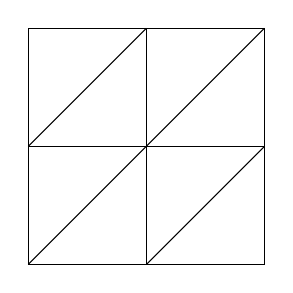
\begin{tikzpicture}[scale=0.5]
\tikzstyle{every node}=[font=\tiny]
      \draw (0,0) -- (6,0) -- (6,6) -- (0,6) -- cycle;
      \draw (0,0) -- (6,6);
      \draw (0,3) -- (6,3);
      \draw (3,0) -- (3,6);
      \draw (0,3) -- (3,6);
      \draw (3,0) -- (6,3);
    \end{tikzpicture}
	\end{center}
  \caption{Initial Mesh with $h=0.5$.}
	\label{fig:Mesh}
\end{figure}


After the FE code is run for each $h$, the corresponding $\psi^h$ is used to calculate the errors $e_0,\, e_1,\text{
and } e_2$, where $e_0,\, e_1,\text{ and } e_2$ are the $L^2,\, H^1,$ and $H^2$ errors respectively, and are
given by
%{\small
\begin{align*}
  e_0 &= \left(\int_{\Omega}\!\left( \psi^h - \psi \right)^2 \,d\mathbf{x}\right)^{\nicefrac{1}{2}}\\
  e_1 &= \left(e_0^2 + \int_{\Omega}\!  \left( \psi^h_x - \psi_x \right)^2 + \left( \psi^h_y - \psi_y \right)^2
    \,d\mathbf{x}\right)^{\nicefrac{1}{2}}\\
  e_2 &= \left(e_1^2 + \int_{\Omega}\!  \left( \psi^h_{xx} - \psi_{xx} \right)^2 + \left( \psi^h_{xy} - \psi_{xy}
    \right)^2 + \left( \psi^h_{yy} - \psi_{yy} \right)^2 \,d\mathbf{x}\right)^{\nicefrac{1}{2}}\\
\end{align*}
%}
The order of convergence, $O$, is then determined by calculating
\begin{equation*}
  O = \dfrac{\log e_{\alpha}^i - \log e_{\alpha}^{i-1}}{\log h_i - \log h_{i-1}},
\end{equation*}
where $e_{\alpha}^i$ is the i$^{th}$ $\alpha$-error corresponding to the i$^{th}$ mesh size, $h_i$.

Additionally, in each of the convergence data tables we also present the number of degrees of freedom (DoFs) for Argyris
Finite Elements. For the uniform mesh as described above and a rectangular domain of length, $L$, and height, $H$, the
DoFs are given by
\begin{equation*}
  %DoF = 6\,\left(\frac{L}{h}+1\right)\,\left(\frac{H}{h}+1\right)+\frac{L}{h}\,\left(\frac{H}{h}+1\right)+\left(2\frac{L}{h}+1\right)\,\frac{H}{h}.
  N = \frac{7h\left(H + L\right) + 9 H L}{h^2} + 6.
\end{equation*}
